\documentclass[12pt]{article}

\usepackage{hyperref}
\usepackage[romanian]{babel}
\usepackage{graphicx}
\usepackage{comment}

\usepackage{lipsum}

\author{Boboi Tomas-Adrian, Cornea Alexandru-Vlad\\ Universitatea Politehnica Timișoara}
\date{Aprilie 2021}
\title{Evaluarea Performanțelor Sistemelor de Calcul\\ Performance Evaluation of Web Services}

\begin{document}
    \maketitle
    \thispagestyle{empty}
    \pagebreak

    \tableofcontents
    \pagenumbering{arabic}
    \pagebreak

    \section{Descrierea sistemului}

        \subsection{Descrierea sistemului din viața reală care se modelează}
            Sistemul modelat în lucrarea aleasă reprezintă o așa-zisă arhitectură orientată pe servicii (Service-oriented Architecture, sau SoA, pe scurt). În cadrul acestei paradigme, serviciile sunt văzute ca entități modulare care pot fi înlănțuite și conectate între ele pentru a obține o funcționalitate nouă, mai complexă decât cea a componentelor individuale care alcătuiesc sistemul.

            Construind un sistem utilizând arhitectura menționată, atât administratorii sistemului, cât și utilizatorii finali, se bucură de beneficii pe care un sistem cu o arhitectură cu un grad de modularitate scăzută nu le poate oferi.

            Pe de o parte, costurile de implementare, îmbunătățire ulterioară, dar și de mentenanță suportate de administratorul de sistem sunt mai scăzute, granularitatea sistemului permițând modificări restrânse pe un modul individual sau un set de module bine definit.

            Pe de altă parte, utilizatorii se bucură de un sistem care oferă o per\-for\-man\-ță mulțumitoare, care poate fi ajustată dinamic, in funcție de diverși factori. Acest lucru asigură îndeplinirea țelului utilizatorului cât mai rapid și mai ușor, fapt ce garantează utilizarea viitoare a serviciului de către client.

            \vspace{\baselineskip}
            \noindent
            Sistemul concret din viața reală care se modelează este o agenție de turism care dorește să-și mute activitatea în mediul on-line. Utilizatorii au acces la această aplicație web prin intermediul unei interfețe, numită \textit{frontend}.

            Utilizatorii aleg mai întâi o locație de pe hartă, după care selectează mijlocul de transport dorit (tren, avion sau taxi).

            Următorul pas este plata, iar utilizatorii care doresc să facă mai multe opriri în călătoriile lor își vor depune călătoria curentă într-un coș de cum\-pă\-ră\-turi. Trebuie menționat aici că aplicația suportă două clase de utilizatori: cei care doresc să planifice o călătorie directă, din punctul A în punctul B, și cei care doresc să-și planifice o călătorie cu opriri intermediare, planificate individual.

            Din cele spuse mai sus, putem deduce serviciile care sunt inlănțuite în cadrul sistemului: \textit{frontend}, \textit{hartă}, \textit{coș de cumpărături}, \textit{tren}, \textit{avion}, \textit{taxi} și \textit{plată}. Imbunătățirea performanței sistemului va presupune imbunătățirea performanțelor serviciilor individuale, fapt ce reprezintă țelul lucrării alese, și al proiectului curent.
            \pagebreak

        \subsection{Descrierea parametrilor care caracterizează sistemul}
            Parametrii care caracterizează sistemul din viața reală sunt timpii de servire ai fiecărui serviciu în parte. Fiecare componentă modulară din sistem are asociat acest timp de servire, care reprezintă timpul scurs între primirea intrării și generarea unei ieșiri spre următorul modul din lanțul sistemului.

            În mod ideal, am dori ca acești timpi să tindă spre zero, însă din considerente de cost și implementare, acest lucru nu este tot timpul posibil. Prețul unui serviciu crește direct proporțional cu calitatea acestuia, astfel încât alegerea în toate cazurile a celor mai performante servicii posibile poate duce la costuri astronomice, care, deși duc la o performanță pe măsură, nu-și justifică costul, clienții neputând sesiza vreo diferență față de un sistem puțin mai ieftin.

            Acesta este unul din scopurile simulării unui asemenea sistem: găsirea combinației de servicii care oferă cea mai bună performanță la prețul cel mai avantajos pentru administratorul de sistem, în funcție de nevoile acestuia și a clienților săi.

            Având în vedere acestea, putem menționa parametrii pe care îi vom folosi pentru a modela și simula sistemul nostru:
            \begin{itemize}
                \item{timpii medii de servire ai fiecărui serviciu}
                    \begin{itemize}
                        \item{servirea se face după o distribuție exponențială, iar acești timpi reprezintă valoarea medie aferentă valorii $\lambda$ care caracterizează distribuția exponențială}
                        \item{timpii de servire corespund fiecărui serviciu în parte, și sunt diferiți în funcție de clasa de utilizatori despre care se discută}
                    \end{itemize}
                \item{probabilitățile de rutare ale serviciului \textit{Frontend}}
                    \begin{itemize}
                        \item{corespondentul lor din viața reală este probabilitatea ca o persoană să acceseze următorul serviciu, pornind de la interfața cu utilizatorul}
                    \end{itemize}
            \end{itemize}
            \pagebreak


    \section{Descrierea modelului construit}

        \subsection{Arhitectura modelului}
            Arhitectura modelului cuprinde serviciile menționate în secțiunea anterioară, modelate ca module de tip \textit{Queue} în contextul programului JMT (Java Modelling Tools). Serviciile sunt următoarele:

            \begin{itemize}
                \itemsep0em
                \item{\textit{Frontend} - interfața cu utilizatorul}
                \item{\textit{Mappe} - serviciul de selectare a unei locații de pe hartă}
                \item{\textit{Carrello} - serviciul care implementează coșul de cumpărături}
                \item{\textit{Aereo}, \textit{Taxi}, \textit{Treno} - serviciile care implementează posibilitatea de a alege între transportul aerian, cu mașina, respectiv cu trenul}
                \item{\textit{Pagamento} - serviciul prin intermediul căruia utilizatorul realizează plata călătoriei, sau a călătoriilor, dacă este un utilizator care alege o călătorie cu mai multe opriri}
            \end{itemize}

            Pe lângă aceste servicii, avem utilizatorii, reprezentați de modului \textit{Utenti}. Aceștia nu mai sunt reprezentați ca un modul de tipul \textit{Queue}, întrucât utilizatorii nu reprezintă un serviciu în sine, ci beneficiarii acestora.

            \begin{figure}[h!]
                \centering
                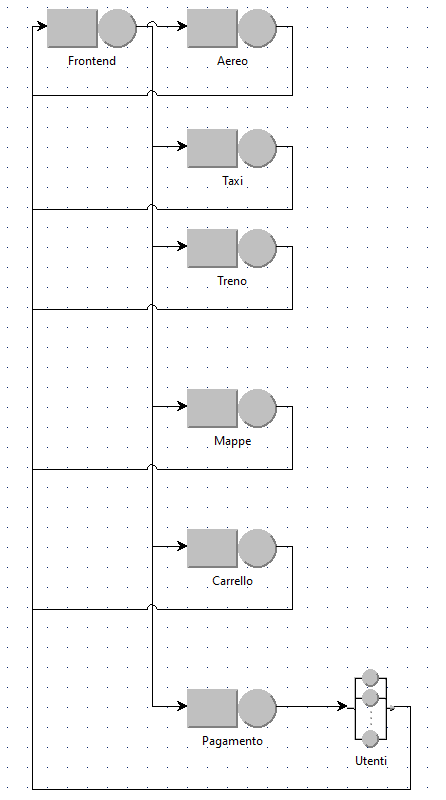
\includegraphics[width=0.5\textwidth]{images/architecture.png}
                \caption{Arhitectura sistemului: utilizatorii accesează prin intermediul interfeței cu utilizatorul diversele servicii oferite de aplicație}
            \end{figure}
            \pagebreak

        \subsection{Indicii de performanță}
            \lipsum[1-2]

        \subsection{Valorile inițiale ale indicilor de performanță}
            \lipsum[1-2]


    \section{Experimente}

        \subsection{Experimentul \#1}
            \lipsum[1-2]
        
        \subsection{Experimentul \#2}
            \lipsum[1-2]

    \section{Concluzii}
        \lipsum[1-2]

\end{document}